\section{J : 2D Arrays \& More Types}
\label{chap:2darrs}

\begin{frame}[fragile]
\frametitle{Initializing 2D Arrays}
\begin{columns}

\begin{column}{0.45\textwidth}
A 2D array is declared as follows:
\begin{verbatim}
#define ROWS 3
#define COLS 5
int a[ROWS][COLS];
\end{verbatim}
%\begin{center}
%\begin{tabular}{|l|l|l|l|l|l|} \hline
    %&   col 1   & col 2 & col 3 & col 4 & col 5 \\ \hline
%row 1   & a[0][0]   & a[0][1]   & a[0][2]   & a[0][3]   & a[0][4] \\
%row 2   & a[1][0]   & a[1][1]   & a[1][2]   & a[1][3]   & a[1][4] \\
%row 3   & a[2][0]   & a[2][1]   & a[2][2]   & a[2][3]   & a[2][4] \\ \hline
%\end{tabular}
%\end{center}
 2D array initialisation :
\begin{verbatim}
int b[2][3] = {1, 2, 3, 4, 5, 6};
int b[2][3] = {{1, 2, 3}, {4, 5, 6}};
int b[ ][3] = {{1, 2, 3}, {4, 5, 6}};
\end{verbatim}
\end{column}

\pause
\begin{column}{0.45\textwidth}
Although 2D arrays are stored in a contiguous block of memory,
we may think of them as a 2D rectangle of data.
\begin{verbatim}
int c[3][5] = {{1,2,3,4,5}, {6,7,8,9,10},
                {11,12,13,14,15}};
\end{verbatim}
\begin{center}
\begin{figure}[h]
%\centerline{
%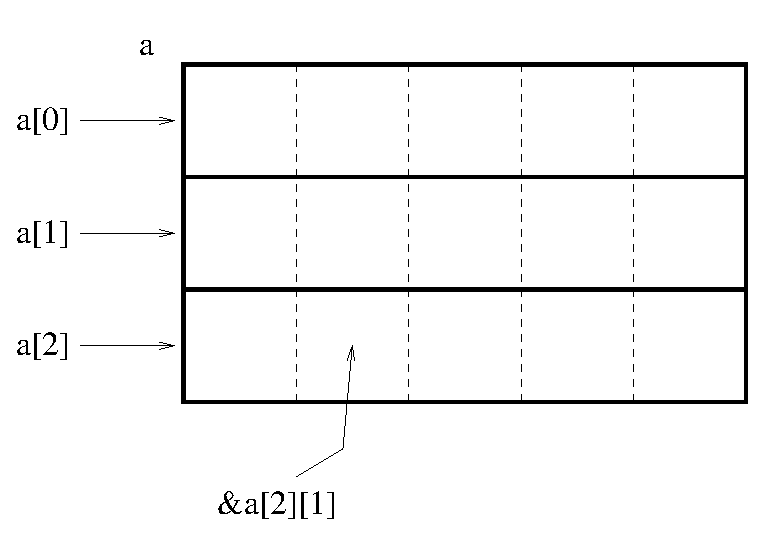
\includegraphics[scale=0.25]{../Figs/array9_3.eps}
%}
\begin{tikzpicture}
\tikzset{arrow/.style={
            thick,
            ->,
            >=latex
        }}
\draw[thick] (0, 0) grid (5, 3);
\foreach \y in {2,...,0}
   \foreach \x in {0,...,4}
      \pgfmathsetmacro\z{int(1+\x+(5*(2-\y)))}
       \node at (\x+0.5,\y+0.5) {\z};
\node (n21) at (-1.0, 3.5) {\tt c[2][1]} ;
\draw[arrow, ocre] (n21.south) -- (1.25, 0.75) ;
\node (n12) at ( 4.0, 3.5) {\tt c[1][2]} ;
\draw[arrow, ocre] (n12.south) -- (2.75, 1.75) ;
\end{tikzpicture}
\end{figure}
\end{center}
\end{column}

\end{columns}
\end{frame}

%%%%%%%%%%%%%%%%%%%%%%%%%%%%%%%%%%%%%%%%%%%%%%%%%%%%%%%%%%%%%%

\begin{frame}[fragile]
\frametitle{2D Distance}

\begin{columns}
\begin{column}{0.60\textwidth}
\lstinputlisting[style=basicc]{../Code/ChapJ/2ddists.c}
\end{column}

\begin{column}{0.30\textwidth}
\outputlisting{../Code/ChapJ/2ddists.autoout}
\end{column}

\end{columns}
\end{frame}


%%%%%%%%%%%%%%%%%%%%%%%%%%%%%%%%%%%%%%%%%%%%%%%%%%%%%%%%%%%%%%

\begin{frame}[fragile]
\frametitle{Cards (again!)}

\lstinputlisting[style=basicc,linerange={68-78},numbers=none]{../Code/ChapJ/cards4.c}

\pause
\begin{itemize}[<+->]
\item The $2D$ arrays of characters here have one string per row.
\item They are of a fixed-width, sometime called {\em ragged-right} or {\em jagged-right} arrays.
\end{itemize}

\end{frame}

%%%%%%%%%%%%%%%%%%%%%%%%%%%%%%%%%%%%%%%%%%%%%%%%%%%%%%%%%%%%%%

\begin{frame}[fragile]
\frametitle{Storage Classes}

\begin{columns}

\begin{column}{0.45\textwidth}
\begin{itemize}[<+->]
\item {\bf auto}
\begin{verbatim}
auto int a, b, c;
auto float f;
\end{verbatim}
Because this is the default, it is seldom used.

\item {\bf extern}

Tells the compiler to look for the variable elsewhere,
possibly another file.

\item {\bf register}

Informs the compiler to place the variable in a high-speed
memory register if possible, i.e.\ if there are enough such
registers available \& the hardware supports this.
\end{itemize}
\end{column}

\pause
\begin{column}{0.45\textwidth}
\lstinputlisting[style=basicc]{../Code/ChapJ/static.c}
\outputlisting{../Code/ChapJ/static.autoout}
\end{column}

\end{columns}
\end{frame}
